\documentclass{article}

% NeurIPS 2025 style, non-anonymous preprint mode (no line numbers). Short version (course limit: 5 pages, 6 if mostly figures).
\usepackage[preprint]{neurips_2025}

\usepackage[utf8]{inputenc}
\usepackage[T1]{fontenc}
\usepackage{hyperref}
\usepackage{url}
\usepackage{booktabs}
\usepackage{amsfonts}
\usepackage{amsmath}
\usepackage{microtype}
\usepackage{xcolor}
\usepackage{graphicx}
\usepackage{siunitx}
\usepackage{caption}
\usepackage{tikz}
\usetikzlibrary{positioning,arrows.meta,fit,calc}

\graphicspath{{figs/}}
\setcitestyle{numbers,square}
\sisetup{group-separator={,},group-minimum-digits=4}
\newcommand{\code}[1]{\texttt{#1}}
\newcommand{\dX}{\Delta X}
\newcommand{\todo}[1]{\textcolor{red}{[#1]}}
% course slides: \sld{Ch7:p19} -> [1, Ch7:p19]
\newcommand{\sld}[1]{\unskip~\cite[#1]{ece284slides}}

\title{Bit-Exact 4-Bit Inference on an $8{\times}8$ Systolic Array:\\
Differential Video Frames, Switchable Dataflow, and Linear Attention}

\author{%
  \todo{Name(s)} \\
  Department of Electrical and Computer Engineering, University of California, San Diego\\
  \texttt{\todo{PID(s)}} \\
}

\begin{document}

\maketitle

\begin{abstract}
We build and verify a 4-bit inference accelerator from training to FPGA. A 4-bit VGG16 with one layer squeezed to $8{\to}8$
channels reaches 91.60\% on CIFAR-10, and that layer runs bit-exactly on an $8{\times}8$ weight-stationary (WS) systolic array
in Verilog. For video, each weight load serves five back-to-back passes (two for the 8-bit key frame, one per 4-bit frame
difference), giving $1.57\times$ fewer cycles with zero error. We also make the array switch to output-stationary (OS) dataflow
at run time ($0.55\times$ EDP on VGG16), run 4-bit linear attention on it (82.09\% ViT accuracy, 144/144 heads bit-exact), and
add zero-operand gating. On a Cyclone IV GX FPGA the three versions run at 75.34, 68.34 and 50.32\,MHz.
\end{abstract}

\section{Introduction}
Getting a low-precision systolic array~\cite{jouppi2017tpu}\sld{Ch7:p12--20} right means matching a trained model, an RTL
datapath and a controller down to the last bit. We go through that flow on a small design (Sec.~\ref{sec:part1}) and then ask
how much more the same $8{\times}8$ array can do: process video as 4-bit frame differences (Sec.~\ref{sec:part2}), switch between
the WS and OS mappings\sld{Ch7:p22--32} per layer (Sec.~\ref{sec:os}), run linear
attention~\cite{katharopoulos2020linear,mcdermott2026lola} (Sec.~\ref{sec:attn}), and gate zero
operands~\cite{moons2017jssc} (Sec.~\ref{sec:zg}).
Table~\ref{tab:summary} summarizes the results; Table~\ref{tab:fpga} gives the FPGA numbers.

\begin{table}[!htb]
\centering
\caption{Summary. FPGA: Quartus Prime Lite 20.1, EP4CGX150DF31I7AD, slow 1200\,mV 100\,\textdegree C corner, power at Fmax
with a 20\% toggle rate. ``Exact'' means bit-identical integers.}
\label{tab:summary}
\small
\begin{tabular}{@{}p{1.9cm}p{5.5cm}p{5.5cm}@{}}
\toprule
 & \textbf{Baseline (Part 1 core)} & \textbf{Differential (Part 2 core)} \\
\midrule
Fmax / power & 75.34 MHz / 462.96 mW & 68.34 MHz / 588.95 mW \\
Accuracy & 91.60\% CIFAR-10 (4b/4b); recovered psum error $3.8\times10^{-6}$ &
  $Y_0$ exact; $Y_1$--$Y_3$ max error 0; no delta saturates \\
Verification & \code{psum.txt} 0/16 mismatches; 60 tiled cases pass &
  \code{y0}--\code{y3.txt} 0/1024 vectors mismatched \\
Passes / cycles & \multicolumn{2}{p{11.2cm}}{4 frames, both modes on the Part 2 RTL: conventional 72 / \num{28079} $\to$
differential \textbf{45} / \textbf{\num{17840}} ($1.57\times$)} \\
\midrule
+$\alpha$ & \multicolumn{2}{p{11.2cm}}{Optimized controller: $1.9$--$2.0\times$ fewer cycles, no RTL change.
WS/OS switch: OS needs $5.2$--$7.3\times$ fewer cycles on narrow layers; $0.55\times$ EDP on VGG16.
Linear-attention ViT: 82.09\%, 144/144 heads exact, 364 cycles/head. Zero gating: same outputs, up to 58\% fewer product
toggles (WS) or 72\% fewer register enables (OS). Final core: 50.32\,MHz, 429.78\,mW.} \\
\bottomrule
\end{tabular}
\end{table}

\section{Baseline: a squeezed 4-bit VGG16 on a weight-stationary array}
\label{sec:part1}
\textbf{Model.} Starting from a 4-bit VGG16~\cite{simonyan2015vgg} on CIFAR-10\sld{Ch4:p17} (91.61\%, PACT activations and STE
gradients\sld{Ch6:p6--7, Ch7:p6--7}), we replace \code{features[27]} with an $8{\to}8$ $3{\times}3$ convolution followed
directly by ReLU (no BatchNorm\sld{Ch4:p13}) and shrink its
neighbours to $256{\to}8$ and $8{\to}512$, keeping the 8 channels with the largest $|\gamma_\text{BN}|$. Accuracy drops to
9.86\% after the cut; 60 epochs of QAT bring it back to \textbf{91.60\%} (Fig.~\ref{fig:train}). The integer result
$\text{ReLU}(\sum w_\text{int}x_\text{int})\Delta_w\Delta_x$\sld{Ch6:p8} matches PyTorch's input to the next layer to $3.8\times10^{-6}$, once TF32
is disabled (TF32 alone causes a $3\times10^{-3}$ error on Ampere GPUs).

\begin{figure}[t]
\centering
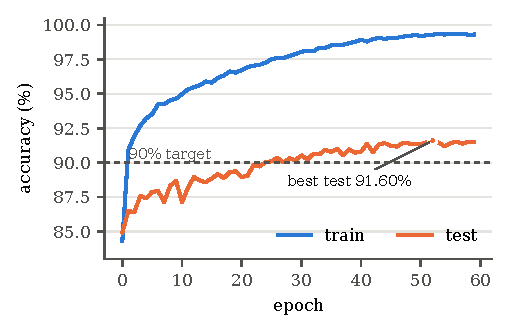
\includegraphics[width=0.42\linewidth]{training_curve.pdf}
\caption{QAT of the squeezed 4-bit VGG16, starting from the HW6 4-bit weights.}
\label{fig:train}
\end{figure}

\begin{figure}[t]
\centering
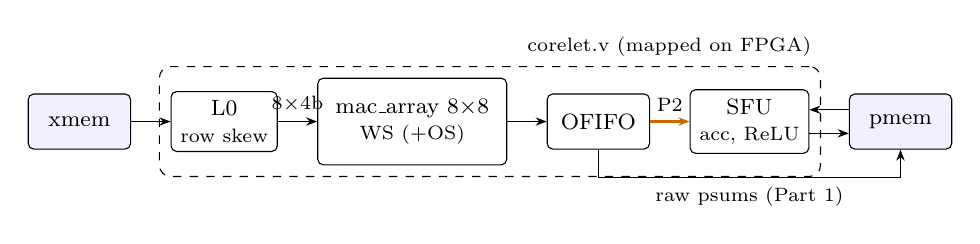
\begin{tikzpicture}[
  font=\footnotesize, >={Stealth[length=4pt]},
  blk/.style={draw, rounded corners=2pt, minimum height=7mm, align=center, fill=white},
  mem/.style={blk, fill=blue!6},
  new/.style={draw=orange!80!black, thick}]
  \node[mem, minimum width=13mm] (xmem) {xmem};
  \node[blk, right=5mm of xmem, minimum width=13mm] (l0) {L0\\\scriptsize row skew};
  \node[blk, right=5mm of l0, minimum width=24mm, minimum height=11mm] (arr) {mac\_array $8{\times}8$\\\scriptsize WS (+OS)};
  \node[blk, right=5mm of arr, minimum width=13mm] (of) {OFIFO};
  \node[blk, right=5mm of of, minimum width=15mm] (sfu) {SFU\\\scriptsize acc, ReLU};
  \node[mem, right=5mm of sfu, minimum width=13mm] (pmem) {pmem};
  \node[draw, dashed, rounded corners=4pt, inner sep=4pt, fit=(l0)(arr)(of)(sfu),
        label={[anchor=south east, font=\scriptsize]north east:corelet.v (mapped on FPGA)}] {};
  \draw[->] (xmem) -- (l0);
  \draw[->] (l0) -- node[above, font=\scriptsize]{8$\times$4b} (arr);
  \draw[->] (arr) -- (of);
  \draw[->, new] (of) -- node[above, font=\scriptsize]{P2} (sfu);
  \draw[->] ([yshift=1.5mm]pmem.west) -- ([yshift=1.5mm]sfu.east);
  \draw[->] ([yshift=-1.5mm]sfu.east) -- ([yshift=-1.5mm]pmem.west);
  \draw[->] (of.south) -- ++(0,-0.35) -| node[pos=0.25, below, font=\scriptsize]{raw psums (Part 1)} (pmem.south);
\end{tikzpicture}
\caption{Datapath. The testbench acts as the controller. Orange: the OFIFO$\to$SFU stream added in Sec.~\ref{sec:part2}.}
\label{fig:block}
\end{figure}

\textbf{Datapath.} Following the course architecture\sld{Ch7:p19, Ch8:p5--6} (Fig.~\ref{fig:block}), weights and
activations enter the array from the west through L0, whose rows are read one cycle apart to create the diagonal
skew\sld{Ch8:p7--21}. During kernel loading each PE keeps the first value it sees before passing the load signal
east\sld{Ch9:p5--9}. The OFIFO collects one output vector per cycle\sld{Ch8:p22}, and the SFU accumulates psums from the psum
SRAM (pmem) with optional ReLU\sld{Ch8:p23}.

\textbf{Verification and schedule.} The testbench runs all seven stages\sld{Ch8:p6} (memory load, kernel load, L0 load, execute, OFIFO to pmem,
accumulate, ReLU) for the 9 kernel positions (kij), against expected files generated from the trained model\sld{Ch10:p9--11}: \textbf{0
mismatches} at every check point, and three injected bugs are caught. A generalized controller loops over channel tiles\sld{Ch8:p3--4}, so any
$3{\times}3$ layer runs on the same RTL; \code{features[24]} (32 input tiles), \code{[27]} and \code{[29]} (64 output tiles) pass
60/60 cases. Execution is only 15\% of the template's 2210 cycles (Fig.~\ref{fig:wave1}), so we rewrote the controller alone to overlap independent
work\sld{Ch9:p2--4} (fill L0 while the kernel loads, drain the OFIFO during execution, prefetch the next weights, fuse ReLU). This gives
1.99$\times$, 1.90$\times$ and 1.94$\times$ fewer cycles on the three layers. The remaining cost is per weight load, which
motivates pushing more activations through each weight load.

\begin{figure}[t]
\centering
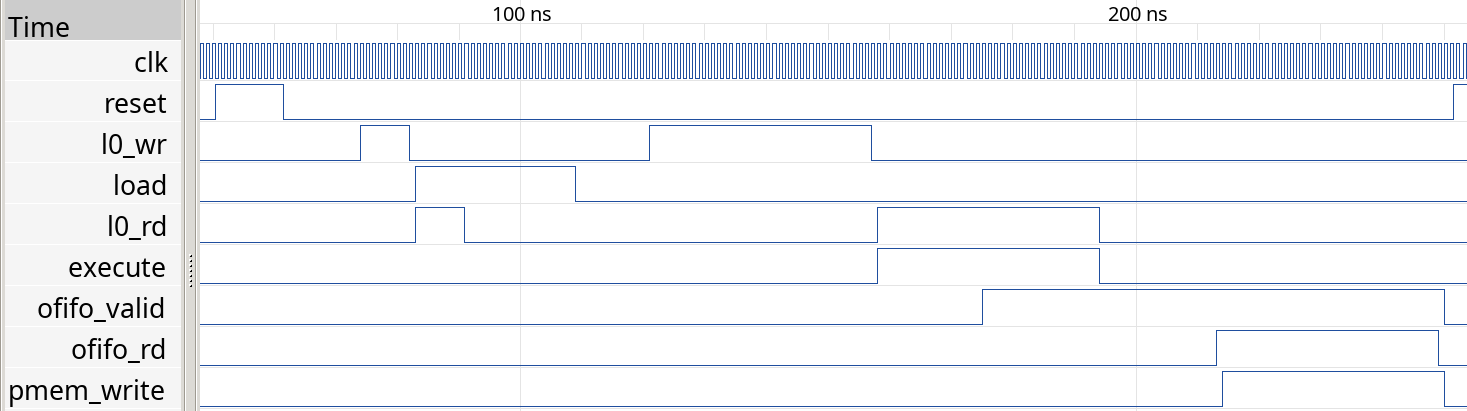
\includegraphics[width=\linewidth]{gtk_part1_kij.png}
\caption{One kij pass, template schedule (GTKWave, \code{core\_tb.vcd}; 1\,ns $=$ 1 cycle; \code{pmem\_write} shown active-high). Execution is a small slice of the pass.}
\label{fig:wave1}
\end{figure}

\section{Differential processing of video frames}
\label{sec:part2}
\textbf{Method.} The four frames X0--X3 hold 2048 signed 8-bit values each; we treat them as $8\times16\times16$ inputs to the
trained \code{features[27]} and compute the raw convolution $Y=W*X$. The key frame is split as $X_0=16X_0^{hi}+X_0^{lo}$ with a
signed high nibble ($X_0\gg4$) and an unsigned low nibble ($X_0\,\&\,15$); a $+128$ offset would turn padding zeros into
non-zeros. Later frames are sent as $\dX_i=\text{sat}_4(X_i-X_0)$, computed by the testbench as the host ($3{\times}2048$
subtract-and-clamps, not in our cycle counts); $X_1$--$X_3$ then cross DRAM$\to$xmem as one nibble instead of two. For each kij the weights load \emph{once}, then five passes
stream through back to back ($X_0^{hi}$ shifted by 4, $X_0^{lo}$, $\dX_1$, $\dX_2$, $\dX_3$), and we reconstruct
$Y_i=Y_0+W*\dX_i$. Conventional 8-bit processing needs 72 passes and 36 weight loads; this needs 45 and 9.

\textbf{Hardware.} The PE gains a signed/unsigned activation mode (cf.\ the HW1 MAC\sld{Ch1:p16} and the signed$\times$unsigned
MAC\sld{Ch6:p12}) that travels with the data, so mixed-mode passes run with no
bubble. The SFU gains a streaming path that adds each OFIFO value (optionally $\ll4$) to its running sum in pmem at one element per
cycle, and a reconstruction path. pmem becomes 1-read/1-write so raw psums never need to be stored (that would take \num{14580}
rows against 2048). Fig.~\ref{fig:wave2} shows the passes in simulation. The largest intermediate value is 6180, so 16-bit accumulators suffice\sld{Ch5:p21}.

\begin{table}[!htb]
\centering\small
\caption{Measured cycles for four frames (same RTL). Compute = kernel loads + execution + OFIFO$\to$SFU$\to$pmem.}
\label{tab:p2cycles}
\begin{tabular}{@{}lrrrrrrr@{}}
\toprule
Method & passes & W loads & execute & DRAM$\to$xmem & compute & recon. & \textbf{total} \\
\midrule
Conventional & 72 & 36 & \num{23328} & \num{2681} & \num{25384} & -- & \textbf{\num{28079}} \\
Differential & 45 & 9 & \num{14580} & \num{1706} & \num{15094} & \num{1026} & \textbf{\num{17840}} \\
Reduction & 1.60$\times$ & 4$\times$ & 1.60$\times$ & 1.57$\times$ & 1.68$\times$ & & \textbf{1.57$\times$} \\
\bottomrule
\end{tabular}
\end{table}


\begin{figure}[t]
\centering
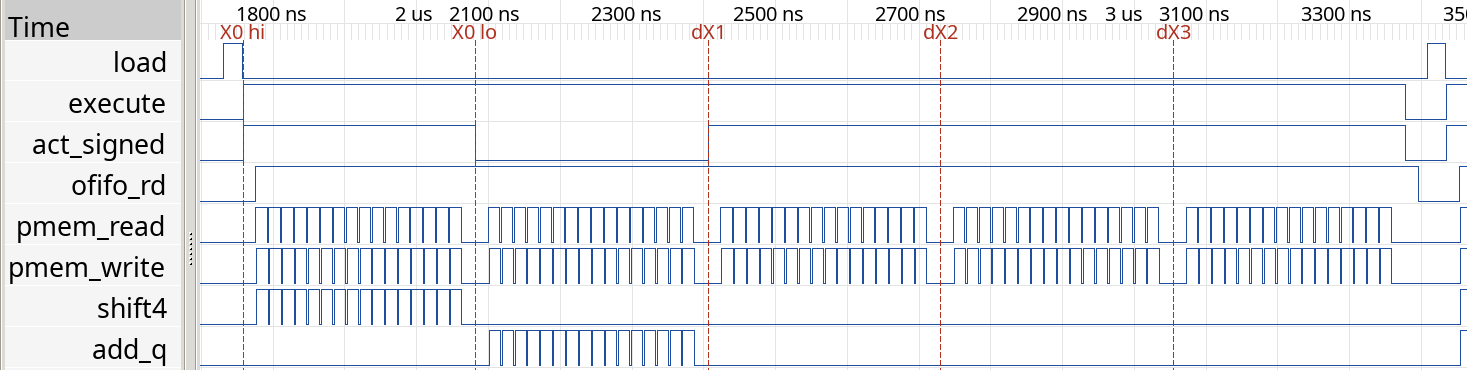
\includegraphics[width=\linewidth]{gtk_part2_kij0.png}\\[3pt]
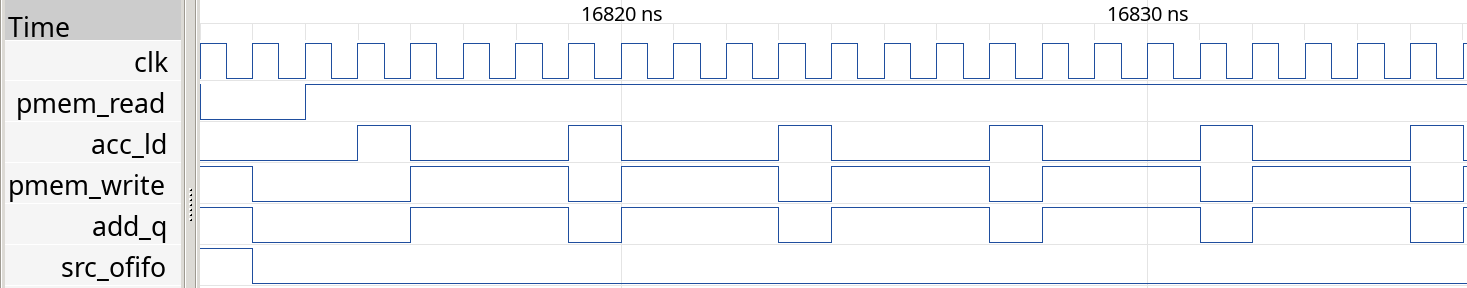
\includegraphics[width=\linewidth]{gtk_part2_recon.png}
\caption{Differential processing (GTKWave, \code{core\_tb\_p2.vcd}; 1\,ns $=$ 1 cycle; pmem enables shown active-high). Top: kij~0, one weight load, then the five passes back to back; \code{act\_signed} is low only for the unsigned X0-low pass. Bottom: reconstruction, 4 cycles per pixel.}
\label{fig:wave2}
\end{figure}

\begin{table}[!htb]
\centering\small
\caption{Accuracy of $Y_i=Y_0+W*\dX_i$ vs.\ 8-bit $W*X_i$ ($Y_0$ is exact).}
\label{tab:p2acc}
\begin{tabular}{@{}lrrrrrr@{}}
\toprule
Frame & $\dX$ zero & $\dX$ saturated & max $|$err$|$ & MSE & SQNR & max $|Y_i|$ \\
\midrule
1 & 22.1\% & 0\% & 0 & 0 & $\infty$ & 6067 \\
2 & 23.1\% & 0\% & 0 & 0 & $\infty$ & 6180 \\
3 & 23.8\% & 0\% & 0 & 0 & $\infty$ & 6003 \\
\bottomrule
\end{tabular}
\end{table}

\textbf{Results.} All 1024 output vectors match the golden files in both differential and conventional mode, and removing the
sign mode or the shift breaks all of them. Every $\dX$ lies in $[-7,7]$, so none saturates and $Y_1$--$Y_3$ equal the 8-bit
references $W*X_i$ exactly (Table~\ref{tab:p2acc}). Because each kij streams 1620 activations, the array is busy 97\% of the time, so
the $1.60\times$ pass reduction becomes a \textbf{1.57$\times$} cycle reduction after reconstruction (Table~\ref{tab:p2cycles}).
The 4$\times$ weight-load saving depends on batching four frames; a large delta (scene cut) would need a new key frame.

\section{Run-time switch between weight- and output-stationary dataflow}
\label{sec:os}
As in the programmable-dataflow chip of\sld{Ch7:p32}, one instruction bit selects the dataflow. In OS mode\sld{Ch7:p25--31} the weight flows north to south on the low 5 bits of the psum wires (idle in
OS, so no new wiring), each PE keeps its own sum\sld{Ch9:p10--13}, and a \code{drain} signal shifts finished sums down into the OFIFO while
clearing them. Weights come from a new weight SRAM through a column-skewed input FIFO. OS runs all three VGG layers and a dense
random matrix product against the same expected files with 0 mismatches. An OS tile costs $K+29$ cycles versus $L+58$ per WS
weight load plus accumulation, so OS needs \textbf{5.2$\times$}, \textbf{7.3$\times$} and \textbf{5.2$\times$} fewer cycles on
f27, f24 and f29. A model calibrated on these costs, with Eyeriss's normalized access energies~\cite{chen2016eyeriss} (buffer
$6\times$, DRAM $200\times$ a 16-bit MAC; a 4-bit MAC costs $1/16$\sld{Ch5:p14}), shows WS winning on conv2--5, where OS's
im2col inputs overflow the on-chip buffer\sld{Ch8:p26} and are re-fetched from DRAM ($2.3$--$2.8\times$ WS's energy).
Choosing per layer gives \textbf{0.55$\times$} the EDP of WS-only (OS-only: 0.58).

\section{Linear attention on the array}
\label{sec:attn}
We train a small CIFAR-10 ViT~\cite{dosovitskiy2021vit} (64 tokens, width 128, 6 blocks, 8 heads, $d_{qk}=8$, $d_v=7$) with
linear attention~\cite{katharopoulos2020linear} $o_i=\phi(q_i)^\top\sum_j\phi(k_j)v_j^\top/\phi(q_i)^\top\sum_j\phi(k_j)$, $\phi=\text{ReLU}$, so all operands
are unsigned 4-bit and a constant-1 value lane produces the normalizer. Following the attention transfer of LoLCATs, as used in LoLA~\cite{zhang2025lolcats,
mcdermott2026lola}, we train a softmax teacher, swap in linear attention and train only $W_q,W_k$ to match it, fine-tune with
distillation, and then run 4-bit QAT with a learned clipping scale per tensor (PACT-style, learning
$\Delta=\alpha/(2^k{-}1)$ directly, with STE gradients\sld{Ch6:p6--7, Ch7:p6--7}) (Table~\ref{tab:vit}).

One head maps to three phases. \emph{A (OS):} accumulate the $8{\times}8$ state $S=\sum_j[v_j|1]\phi(k_j)^\top$; each drained
row is already a WS kernel word, so no transpose is needed. \emph{R:} the SFU requantizes $S$ with a shared exponent (block
floating point, which cancels in the division). \emph{B (WS):} stream the queries with $S$ as the kernel and divide in the SFU;
since the attention weights are non-negative and sum to 1, the output fits in 4 bits and the divider needs only 4 steps. The RTL
matches the model on \textbf{144/144 heads} and takes \textbf{364 cycles} per head, versus $\approx$3256 for softmax on the same
array, a gap that grows with sequence length (Fig.~\ref{fig:attn}). Caveat: without attention the ViT still reaches 81.89\% (Table~\ref{tab:vit}), so attention adds only
1--1.4 points here; this shows the mapping is exact and cheap, not that the task needs attention.

\begin{figure}[!tb]
\begin{minipage}[t]{0.5\linewidth}
\vspace{0pt}\centering\small
\captionof{table}{Tiny ViT accuracy on CIFAR-10.}
\label{tab:vit}
\begin{tabular}{@{}lr@{}}
\toprule
Stage & accuracy \\
\midrule
softmax teacher (float) & 83.31\% \\
linear swapped in, untrained & 56.05\% \\
after attention transfer & 80.48\% \\
fine-tuned (float) & 82.93\% \\
4-bit QAT & 82.40\% \\
\textbf{4-bit, bit-exact HW attention} & \textbf{82.09\%} \\
\midrule
ablation: no attention / uniform & 81.89 / 81.41\% \\
\bottomrule
\end{tabular}
\end{minipage}\hfill
\begin{minipage}[t]{0.47\linewidth}
\vspace{0pt}\centering
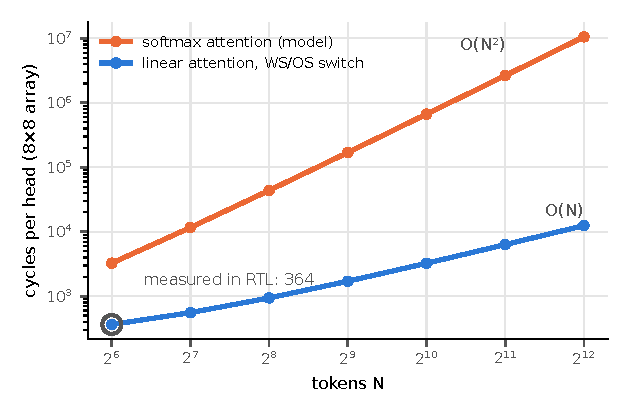
\includegraphics[width=0.9\linewidth]{alpha_attn_scaling.pdf}
\captionof{figure}{Attention cycles per head vs.\ tokens (linear: measured at $N=64$; softmax: modelled).}
\label{fig:attn}
\end{minipage}
\end{figure}

\section{Zero-guard gating and FPGA results}
\label{sec:zg}
Following the guard-bit gating of Moons and Verhelst~\cite{moons2017jssc}\sld{Ch10:p3--5}, each operand carries a guard bit
set when it is zero (zeros come from ReLU and quantization\sld{Ch9:p17}). In WS a guarded activation is not latched, which freezes the multiplier;
in OS the operand is forced to 0 and the accumulator is not enabled. (Merely holding the operand in OS \emph{increased} toggles,
because the stale activation meets a moving weight; cf.\ the limits of gating\sld{Ch10:p5}.) Outputs are identical with gating on or off. Table~\ref{tab:zg} shows the
savings land in different places: the multiplier in WS, the accumulator in OS. The dense control shows none.

\begin{table}[!htb]
\centering\small
\caption{Zero gating: change vs.\ gating off over all 64 PEs. ``Reg.\ enables'' are what clock gating would remove.}
\label{tab:zg}
\setlength{\tabcolsep}{4pt}
\begin{tabular}{@{}llrrr@{}}
\toprule
Workload & flow & zero MACs & product toggles & reg.\ enables \\
\midrule
VGG f27 / f24 / f29 & WS & 80--88\% & $-48$ / $-58$ / $-52\%$ & $-9\%$ \\
VGG f27 / f24 / f29 & OS & 76--84\% & $0\%$ & $-66$ / $-72$ / $-61\%$ \\
Part 2 delta frames & WS & 34.3\% & $-22\%$ & $-6\%$ \\
ViT attention, layer 0 & OS+WS & 44.9\% & $-17\%$ & $-14\%$ \\
Dense random (control) & OS & 0\% & $0\%$ & $0\%$ \\
\bottomrule
\end{tabular}
\end{table}

\begin{table}[!htb]
\centering\small
\caption{FPGA results for \code{corelet} (slow 1200\,mV corner; power at Fmax, 20\% toggle rate). ``Final'' includes Secs.~\ref{sec:os}--\ref{sec:zg}.}
\label{tab:fpga}
\setlength{\tabcolsep}{4pt}
\begin{tabular}{@{}lrrr@{}}
\toprule
 & Baseline & Differential & Final \\
\midrule
LEs fitted / registers / pins & \num{17326} / \num{11937} / 426 & \num{29686} / \num{12624} / 431 & \num{27782} / \num{15678} / 346 \\
\textbf{Fmax} at 100\,\textdegree C ($-40$\,\textdegree C) & \textbf{75.34} (85.61) MHz & \textbf{68.34} (78.28) MHz & \textbf{50.32} (57.0) MHz \\
\textbf{Power} @ Fmax (I/O share) & \textbf{462.96} mW (39\%) & \textbf{588.95} mW (33\%) & \textbf{429.78} mW (26\%) \\
\bottomrule
\end{tabular}
\end{table}

In all three designs Fmax is set by a path to the output pins that exists only because the corelet is the FPGA top level; the
internal limits are $\approx$114, 118 and 84\,MHz. All Part 2 RTL changes add only 5\% LEs after synthesis
(\num{22343}$\to$\num{23465}); the fitted jump is mostly the fitter duplicating OFIFO read-mux registers for timing on the
new OFIFO$\to$SFU path. The final design reached
only 32.3\,MHz until we pipelined the divider over two stages (+2 cycles per head); its 64 MACs map to DSP blocks, and pin
count falls to 346 (473 before we moved the pmem write mux inside the corelet).

\textbf{Limitations.} The workloads are small, exactness needs unsaturated deltas, EDP and softmax figures are modelled, and
FPGA power is vectorless, so gating savings are given as toggle counts.

{\small
\begin{thebibliography}{99}\setlength{\itemsep}{1pt}
\bibitem{ece284slides} M.~Kang. ECE~284 lecture slides, Ch.~1--10. UC San Diego, Fall 2026.
\bibitem{jouppi2017tpu} N.~P. Jouppi et~al. In-datacenter performance analysis of a tensor processing unit. \emph{ISCA}, 2017. [Slides Ch7:p12]
\bibitem{chen2016eyeriss} Y.-H. Chen, J.~Emer, and V.~Sze. Eyeriss: A spatial architecture for energy-efficient dataflow for
convolutional neural networks. \emph{ISCA}, 2016. [Slides Ch4:p10]
\bibitem{moons2017jssc} B.~Moons and M.~Verhelst. An energy-efficient precision-scalable {ConvNet} processor in 40-nm {CMOS}.
\emph{IEEE JSSC}, 2017. [Slides Ch9:p19, Ch10:p3--4]
\bibitem{simonyan2015vgg} K.~Simonyan and A.~Zisserman. Very deep convolutional networks for large-scale image recognition.
\emph{ICLR}, 2015. [Slides Ch5:p3]
\bibitem{mcdermott2026lola} L.~McDermott, R.~W. Heath~Jr., and R.~Parhi. {LoLA}: Low-rank linear attention with sparse caching.
\emph{TMLR}, 2026.
\bibitem{katharopoulos2020linear} A.~Katharopoulos et~al. Transformers are {RNNs}: Fast autoregressive transformers with linear
attention. \emph{ICML}, 2020. [Cited in LoLA]
\bibitem{zhang2025lolcats} M.~Zhang et~al. {LoLCATs}: On low-rank linearizing of large language models. \emph{ICLR}, 2025. [Cited in LoLA]
\bibitem{dosovitskiy2021vit} A.~Dosovitskiy et~al. An image is worth 16x16 words: Transformers for image recognition at scale.
\emph{ICLR}, 2021.
\end{thebibliography}
}

\end{document}
